%% CHAPTER 2 (probably)
%% HCHO Levels

\chapter{TODO: move to biogenic isop chapter: Formaldehyde product over Australia} % Main chapter title
\label{ch_HCHO} %better reference name like ch_HCHO

%%----------------------------------------------------------------------------------------
%%	SECTION
%%----------------------------------------------------------------------------------------  
\section{Satellite HCHO measurements}
\label{ch_HCHO:sec:satelliteHCHO}
  \subsection{Satellite Retrievals}
  
  \subsection{Air Mass Factors}
    \label{ch_HCHO:sec:satelliteHCHO:AMFs}
    
  
  \subsection{OMI HCHO data products}
    
  
  \subsection{HCHO Vertical Column Calculation}
    \label{ch_HCHO:sec:satelliteHCHO:CalculationOfVC}

    
  \subsection{Uncertainty in OMI total columns (Moved)}
  \label{ch_HCHO:sec:OMIuncertainty}
    % Moved to BioIsop
    \ref{ch_HCHO:sec:OMI_uncertainty_calculation}.
    
  \subsection{Reference sector correction for comparison of products to various models}
    
%----------------------------------------------------------------------------------------
%	BVOC FROM HCHO SECTION
%----------------------------------------------------------------------------------------
\section{Recalculating HCHO from satellite(OMI) data over Australia}
\label{ch_HCHO:sec:creatinginventory}

  \subsection{Process Outline}
    
    
    
    
    
    

  \subsection{Quality filtering OMI HCHO slant columns}
    \label{ch_HCHO:sec:OMIFiltering}
    %% TODO: Quality flags and cloud cover metric uses, and discussion, along with statistics like how many datapoints are removed.
    
    
  
    
  \subsection{Reading OMHCHO daily slant columns}
    
    
    TODO: Show an example of OMI swaths.
    
  \subsection{Regridding to 0.25 by 0.3125 8-day averaged vertical columns}
    

  \subsection{Filtering pyrogenic HCHO}
  \label{ch_HCHO:sec:filteringfires}
    TODO: How modis fire counts are used as well as statistics on removed data points.
    
    
    An example of the change in resolution is provided in figure \ref{ch_HCHO:fig:modisgridspace}, where the grids are shown over a basic map of Tasmania.
    The direct affect of this interpolation is shown as an example in figure \ref{ch_HCHO:fig:modisinterpolation}, which is showing the regridded MODIS fire count over Australia from January 2005 (avg of first 8 days) in two subplots.
    
    \begin{figure}[!htbp]\begin{center}
      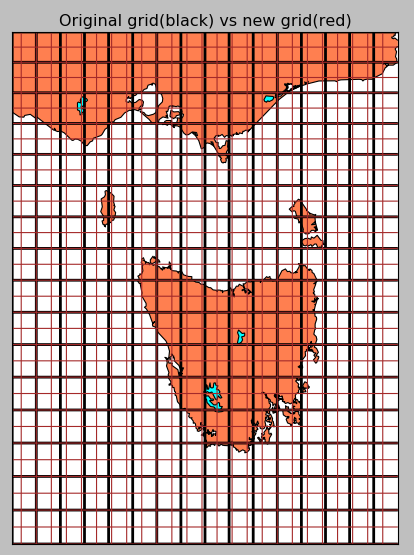
\includegraphics[width=0.7\textwidth]{Figures/MODIS_grid_space.png}
      \caption{Example of grid space change using 0.5x0.5 and 0.25x0.3125 latitude by longitude resolution.}
      \label{ch_HCHO:fig:modisgridspace}
    \end{center}\end{figure}
    
    \begin{figure}[!htbp]\begin{center}
      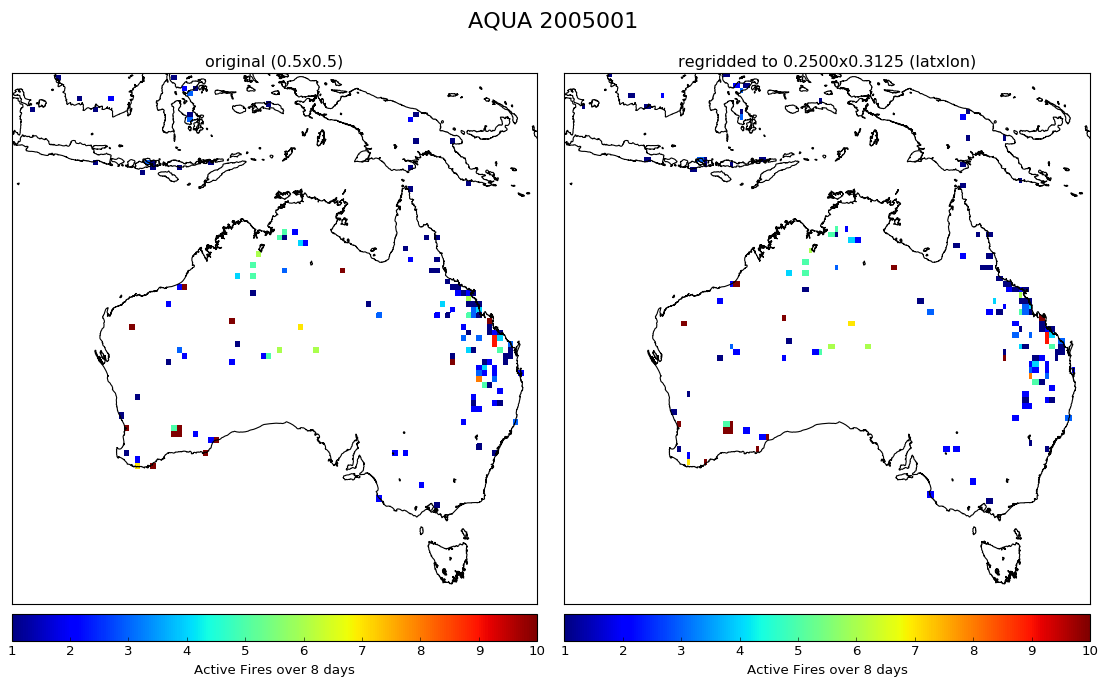
\includegraphics[width=\textwidth]{Figures/MODIS_Regrid_Comparison.png}
      \caption{Example of MODIS 8 day grid interpolation from 0.5x0.5 to 0.25x0.3125 latitude by longitude resolution.
      This example uses MODIS fire counts for 1-8 January 2005.}
      \label{ch_HCHO:fig:modisinterpolation}
    \end{center}\end{figure}
    
    
    
  \subsection{Filtering anthropogenic HCHO}
    TODO
  
  \subsection{Recalculating the AMF to create our own vertical HCHO columns}
  \label{ch_HCHO:sec:recalculating_AMF_description}
    OMI's apriori shape factor is based on the GEOS-Chem (v9) model, which uses 47 layers between the earth's surface and the top of the atmosphere using a pressure-eta hybrid (the actual values are shown in table \ref{app_a:tab:gc_47_vgrid}).
    Taking a more recent GEOS-Chem apriori shape factor and integrating along the vertical axis using equation \ref{ch_HCHO:eqn:AMFintwSdz} gives us a new AMF (AMF$_n$).
    Since we are using the $\omega$ provided by OMI, we remove the AMF$_G$ term from this calculation.
    The integration is done in Python using a simple rectangular method, which multiplies the integrand midpoints by the change in height, and then takes the sum.
    This is identical to calculating the integral if we assume the integrand is linear between each measured point, and introduces no new uncertainty.
    All that remains for recalculating the total vertical column using our new apriori shape factor is to apply the new AMF and remove the old:
    \begin{equation*}
      \Omega_{new} = \Omega \frac{AMF}{AMF_n}
    \end{equation*}
    
    The vertical column scattering weights and apriori shape factors provided in the OMHCHO dataset are defined on 47 levels.
    In order to reformulate the vertical column using updated GEOS-Chem hcho apriori shape factors I have run GEOS-Chem version 10.01 on the full 72 level vertical grid at 2 by 2.5 (lat by lon) degree monthly resolution. 
    The simulated vertical profiles of HCHO are averaged from 1300-1400 local time in order to match the satellite overpass time of roughly 1330.
    These vertical profiles then provide the apriori shape factor for the higher horizontally resolved satellite columns, which pick the nearest apriori from the model.
    TODO: determine which of these is correct!
    a)The new apriori profiles are monthly averages, which is the same temporal resolution used by the OMI apriori shape factors.
    b)The new apriori profiles are simulated daily and averaged over 8 days along with the recalculated total vertical columns.
    
    A new AMF is determined using equation \ref{ch_HCHO:eqn:AMFintwSdz}) with the apriori shape factor set by our GEOS-Chem model run.
    In order to reformulate the AMF, GEOS-Chem's 72 level vertical profile is transformed from ppb to a normalized number density profile in order to match equation \ref{ch_HCHO:eqn:ShapeFactor}. 
    This conversion uses the following equation: 
    \begin{equation} \label{ch_HCHO:eqn:ppbto}
      \eta_{HCHO} = ppb_{HCHO} \times \eta_a \times 10^{-9}
    \end{equation}
    where $\eta_{HCHO}$ is the number density of a HCHO, and ppb$_{HCHO}$ is the molecules of that species per billion molecules of air.
    In order to normalize these vertical density profiles over the globe, we divide by the modelled total vertical column $\Omega_{HCHO}$ which is determined by:
    \begin{equation*}
      \Omega_{HCHO} = 2.12\times 10^{13} \Sigma_z \left( ppb_{HCHO}(z) (P(z)-P(z+1)) \right)
    \end{equation*}
    where P(z) is the pressure (hPa) at the bottom of altitude level z, the constant 2.12e13 is determined from equation (TODO: run through this number in another section?).
    In effect this equation sums over the molecules per cm$^2$ in each altitude level.
    
    We have S$_z(z)$ and $\omega(z)$ over the vertical pressure coordinate z at all latitude and longitude points on whatever grid we wish. 
    A conversion to the sigma ($\sigma$) vertical coordinate is performed using $ P = \sigma (P_S - P_T) + P_T$, where $P_T$ is pressure at the top of the atmosphere and $P_S$ is surface pressure.
    In the sigma coordinate system we calculated the shape factor as follows:
    \begin{equation} \label{ch_HCHO:eqn:ShapeFactorSigma}
      S_\sigma(\sigma) = \frac{\Omega_a}{\Omega_v}C_{HCHO}(\sigma)
    \end{equation}
    where $\Omega_a$ is the vertical column of air from the surface to the top of the atmosphere and C$_{HCHO}(\sigma)$ is the mixing ratio of HCHO.
    This equation comes from \citet{Palmer2001}, and is unitless since $\Omega_a / \Omega_v$ is molecules of air per molecule of HCHO; the opposite of $C_{HCHO}$.

    Pressure dimension from OMI are the surface pressures from each gridbox (offline conversation with Dr Christopher Miller).
    Determining the geometric pressure midpoints (here onwards pressure levels) and interpolating to our increased vertical resolution involves a few steps.
    The lowest level (with highest pressure) in whichever pressure dimension (ours or OMI's) extends to the lowest altitude (or highest pressure) is interpolated upwards to match the lowest level in the other dimension.
    Secondly, if the OMI dimension has been changed, the scattering weights are interpolated onto this updated dimension.
    Figure \ref{ch_HCHO:fig:AMF_Surface_Relevel} shows how these first two steps are applied using three fake array comparisons and updating the array with the lower surface level.
    Finally, once our dimensions match at the surface (we are not so worried about the very top of the atmosphere) we interpolate the scattering weights onto our updated GEOS-Chem pressure dimension.
    
    \begin{figure}[!htbp]
      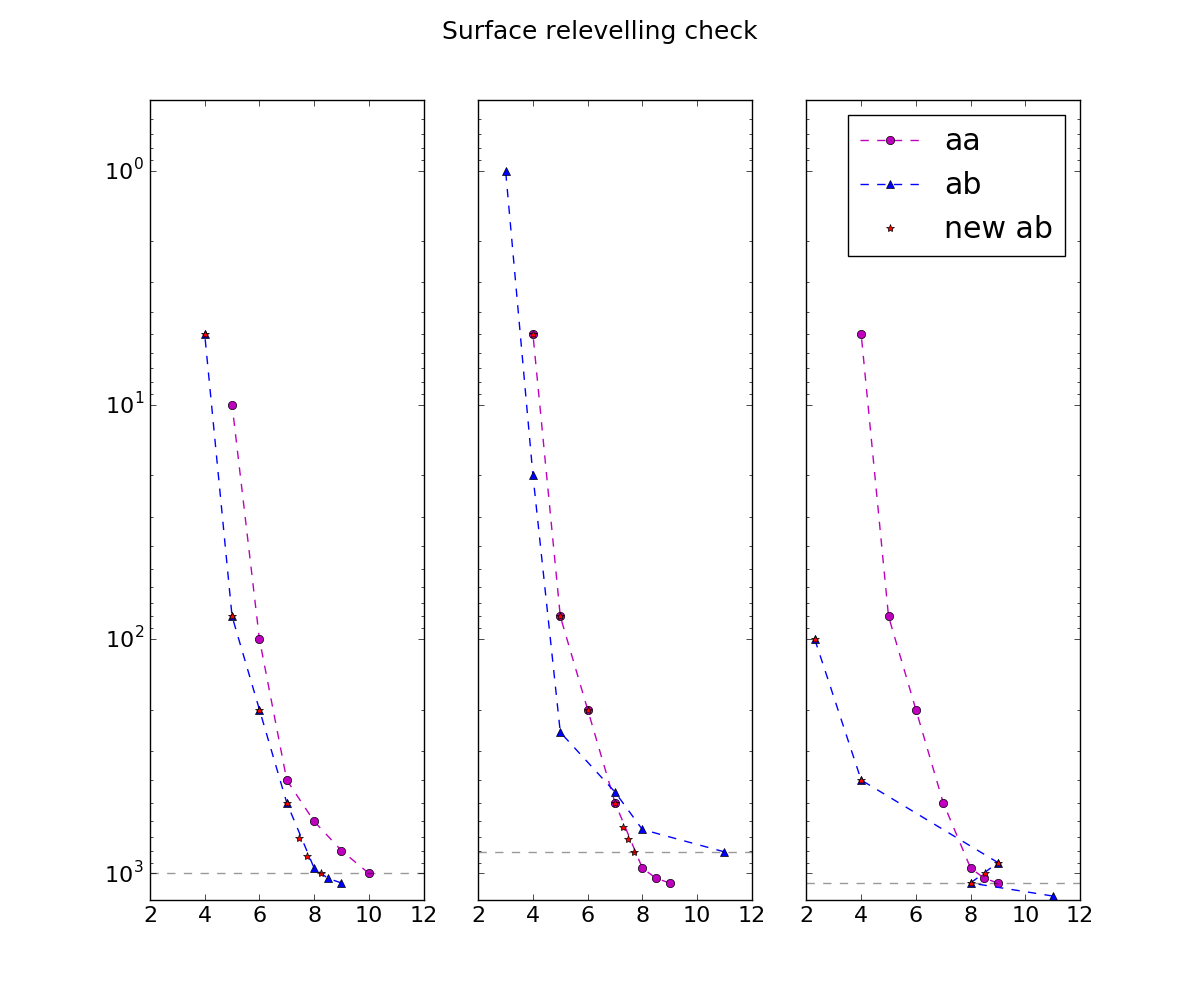
\includegraphics[width=\textwidth]{Figures/HCHO/SurfaceRelevelCheck.png}
      \caption{Constructed example of the initial interpolation of OMI's $\omega$ onto a pressure dimension with mismatched surface pressure.}
      \label{ch_HCHO:fig:AMF_Surface_Relevel}
    \end{figure}
    
    %If I change this to use an inverted geometric midpoint calculation then I need to explain it, otherwise I will need to note the assumption
    %$ \sqrt{ \left( P_1 \times P_{surf} \right)} = P_0 $
    %becomes $ P_{surf} = \frac{P_0^2}{P_1} $ where currently I'm using $P_0$ as the surface.

    S$_\sigma(\sigma)$ Is determined after running GEOS-Chem, which outputs vertical profiles of air density and HCHO mixing ratio, at 72 vertical levels with associated metadata such as vertical layer height and pressure, grid box location, height, and surface pressure.
    Using these outputs the vertical columns ($\Omega_a, \Omega_v$) are calculated for each horizontal grid point (i, j) as follows:
    \begin{align*}
      \Omega_a(i,j) &=& \Sigma_z \left( N_a(i,j,z) \times H(i,j,z) \right)
      \\
      \Omega_z(i,j) &=& \Sigma_z \left( N_{HCHO}(i,j,z) \times H(i,j,z) \right)
    \end{align*}
    where $N_a$, and $N_{HCHO}$ are the densities of air and HCHO, H is the layer height (for each grid box).
    Note that HCHO density is determined from the outputted mixing ratio: $N_{HCHO} = C_{HCHO} \times N_a$.

    S$_\sigma(\sigma)$ is then stored in HDF-EOS5 format, to be used in conjunction with the satellite measurements to calculate an AMF as shown in equation \ref{ch_HCHO:eqn:AMFintwSdz}.
    As the GEOS-Chem V10.01 output is in bitpunch format, the code to read the data and create the shape factor is written in IDL, which has many procedures and functions which are already written to handle reading this format (provided by GAMAP).
    The code is provided in supplementary TODO: put code into supplement section.
    
    For each OMI slant column, a new AMF is calculated using S$_\sigma(\sigma)$ and the provided scattering weights $\omega(\sigma)$ using equation \ref{ch_HCHO:eqn:AMFintwSdz}.
    This integral is applied in python by taking the sum of S$_\sigma(\sigma) \times \omega(\sigma) \times \mathrm{d}\sigma$ for each $\sigma$ determined at 72 levels in GEOS-Chem, with the provided $\omega$ interpolated linearly to these same levels.
    An example of these interpolations is shown in figure TODO: interpolation figure with symbols at original points and interpolated line overplotted for both functions over hPa.
    Globally this reprocessing changed the AMF by TODO: global total percent difference in AMF. 
    In total this caused TODO: total column HCHO change globally/yearly
    In Summer over Australia the global AMF difference was TODO: Difference summers only.
    This changed Australia's HCHO amounts from TODO: X to Y Tg per year plus minus one std.
    
  \subsection{AMF code from Paul Palmer}
  \label{ch_HCHO:sec:PPCode}
    TODO: describe how I use this here
    I use code originally written by Dr. Paul Palmer with various updates and modifications described in section (TODO:) as another way to recalculate the AMF using information from the satellite swaths and the GEOS-Chem overpass simulation output.
    These are used to recalculate the instrument sensitivity or scattering weights for each pixel, as well as the shape factor which together are integrated to give the pixel AMF.
   
   GEOS-Chem outputs quantities averaged between 1200 and 1400 LT, including optical depths at several wavelengths (TODO: list), dust, and HCHO.
   I run a script on the satellite swaths which pulls out a subset of the pixel information into a daily csv file, which can be read by the AMF code as modified by Dr. Luke Surl, in conjunction with the GEOS-Chem outputs for each day.
   The AMF code is then run and produces a csv of recalculated AMFs which get read by my python code and associated with the corresponding pixel.
    
  \subsection{Determination and application of the pacific ocean reference sector normalisation}
    \label{ch_HCHO:sec:RSC}


    
  \subsection{Estimation of error or uncertainty (moved to Bioisop)}
  %\label{ch_HCHO:sec:OMI_uncertainty_calculation}
    % moved to BioIsop
    
  
\section{Validation and comparisons}
  \label{ch_HCHO:sec:Validation}
  
  \subsection{Comparison with standard OMI product}
    Figure TODO: shows global and Australian HCHO eight day averaged total column maps for 1-8 January 2005, along with the reduced major axis (RMA) regression corellation and percentage difference.
   This comparison shows how reprocessing with an updated model can have a systematic influence on the total column.
  
  \subsection{Comparison with in-situ measurements}
    TODO: Describe Wollongong FTIR and junk
    Analyse comparison of gridbox with instrument!

  \subsection{Summary}
    First the OMI HCHO level 2 data was downloaded, and read using python creating a list of good pixels for each day.
    Next the associated AMF and reference sector correction for each good pixel was calculated using GEOS-Chem for the apriori shape factor, and using the provided scattering weights from OMI.
    Each 8 days the pixel list is averaged onto a 0.25$^{\circ}$ latitude by 0.3125$^{\circ}$ longitude grid.
    The new HCHO product along with counts and average uncertainty of pixels used in the grid square is also kept.
    The product includes the 8-day gridded averages of the old and new AMFs, the average correction sector from GEOS-Chem over the pacific ocean, and the old and new HCHO with and without the reference sector correction from \cite{Abad2015} applied.
    
    \subsection{Conclusions}
